\chapter{Zielspezifikation ( 5 \%)}

Wie das letzte Kapitel gezeigt hat,
bringen bisherige Systeme diverse Probleme mit sich.
Da diese nicht oder nur schwer innerhalb dieser Systeme l\"osbar sind,
soll ein neues System geschafen werden.

Dieses Kapitel soll die entsprechenden Ziele qualitativ und quantitativ festlegen.




% tests in sektionen mit angeben

% zeitanforderungen ?!

% funktional, tests, szstemanforderunge? bessereer name
% abgrenzungen



\section{Systemanforderungen}

Die Systemanforderungen legen funktionale Eigenschaften der Software auf Systemebene fest.
Dabei werden 3 Punkte als wichtig erachtet.


\begin{description}

\dhitem[S1]
Das System darf sich nicht vom Absturz/Fehlerfall einzelner Komponenten st\"oren lassen.
Jederzeit muss es m\"oglich sein, Teile des Systems hart zu beenden oder
die Struktur des Systems zu ver\"andern.

\dhitem[S2]
Alle anfallenden L\"angerfristig verf\"ugbaren Daten m\"ussen mittels einer Standardschnittstelle
f\"ur Datenbankzugriff abfragbar/verwendbar sein.

\dhitem[S3]
Das System soll offen f\"ur Erweiterungen stehen,
und soweit m\"oglich Erweiterbarkeit aktiv unterst\"utzen.
\end{description}


\section{Funktionenale Anforderungen und Use Cases}
% kann/soll kriterien

Um ein modernes und erweiterbares CI-System zu schaffen,
m\"ussen zuerst die Kernfunktionen festgelegt werden.
Anschliessend kann auf dieser Basis
eine Platform f\"ur Erweiterungen geschaffen werden.
Dabei ist schon im Kern das bereits Angesprochene Problem
der Matrix-Builds zu beachten.

Anschliessend K\"onnen auf dieser Basis n\"utzliche weiterf\"uhrende Funktionen
sowie die gew\"unschten Erweiterungen geschaffen werden.


\subsection{Kernfunktionen}

Die Kernfunktionen bilden das absolute Minimum an Funktionen.
Jede von ihnen ist unabdingbar.

\begin{figure}[ht]
  \centering
  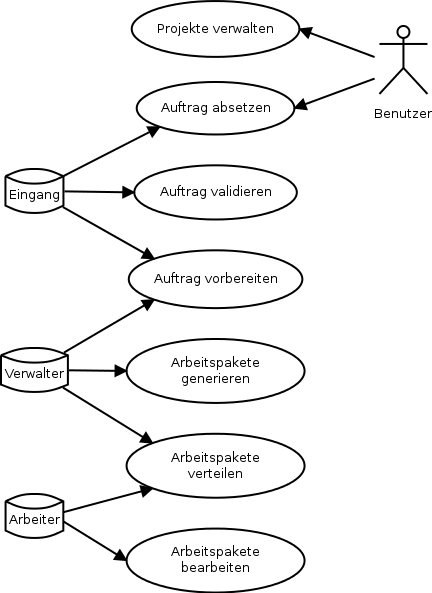
\includegraphics[width=0.7\textwidth]{imageinput/use-case-muss.png}
  \caption{\"Ubersicht Use-Cases - Kern}
  \label{fig:use-case-muss}
\end{figure}

Wie in Abbildung~\ref{fig:use-case-muss} gut zu erkennen,
stellt sich der Absolute Kern eines CI-Systemes aus relativ wenigen Funktionalit\"aten zusammen.

Die erste Notwendige Funktion stellt die Verwaltung von Projekten \deffeat{feat:projekt-verwalten}.
Sind diese dann angelegt, mann man damit beginnen, Auftr\"age abzusetzen \deffeat{feat:auftrag-absetzen}.
Ist ein Auftrag abgesetzt, so muss seine Richtigkeit sichergestellt werden \deffeat{feat:auftrag-validieren},
danach kann er f\"ur die Bearbeitung \deffeat{feat:auftrag-vorbereiten} vorbereitet werden.

Nach dem der Auftrag an sich vorbereitet ist, m\"ussen entsprechend der Build-Matrix \deffeat{feat:auftrag-matrix}
Arbeitspackete generiert werden \deffeat{feat:arbeitspacket-generieren}.
Diese Arbeitspackete werden anschliesend verteilt \deffeat{feat:arbeitspacket-verteilen} und abgearbeitet \deffeat{feat:arbeitspacket-abarbeiten}.

Das Abarbeiten der Arbeitspackete sollte in Schritten erfolgen \deffeat{feat:arbeitspackete-schritte},
wobei die grundlegendste Art von Arbeitsschritt das Ausf\"uhren eines Prozesses \deffeat{feat:arbeitsschritt-prozess} ist.


\subsection{Weiterf\"uhrende Funktionen}

Nach dem Umsetzung des funktionalen Kerns als Basis,
k\"onnen nun weiterf\"uhrende Funktionen angelagert werden.
Diese sind nicht zwingend notwendig, tragen jedoch erheblich dazu bei,
informierte Entscheidungen \"uber den Zustand eines Projektes in Integration zu treffen.

\subsubsection{Datensammlung}

Zun\"achst einmal gilt es Datensammlung beim Ablauf eines Arbeitschrittes zu betrachen.
\"Ublicherweise muss zumindest STDOUT/STDERR schon zur Laufzeit festgehalten \deffeat{feat:arbeisschritt-stdio} werden.
Weiterhin besteht auch Interesse an statistisch auswertbaren Daten
wie z.B. den Speicherverbrauch \deffeat{feat:arbeitsschritt-stats}.

Auch nach dem Ausf\"uhren eines Arbeitschrittes fallen interessante Daten an.
Oftmals sorgt zumindest einer der Arbeitschritte f\"ur das Generieren eines Ausf\"uhrbaren Programmes.
Dieses sollte sp\"ater auch zur Verf\"ugung gestellt werden \deffeat{feat:arbeitsschritt-artefakt}.
Weiterhin finden sich Testresultate in diversen Standardformaten \deffeat{feat:arbeitsschritt-resultate},
wie z.B. JunitXML.

\subsubsection{Arten Arbeitsschritte}

Auch bei den Arten der Arbeitsschritte gibt es f\"r gew\"ohnlich mehrere M\"oglichkeiten (siehe \Cref{chap:ist-analyse}).
Neben den gewohnten Prozessschritten (\cref{feat:arbeitsschritt-prozess}) sind weitere Arten \"ublich.
Interaktion mit dem Quellcodemanagement \deffeat{feat:arbeitsschritt-scm}, sowie
Schritte implementiert in einer Scriptsprache \deffeat{feat:arbeitsschritt-script},
stellen weiterf\"uhrende Hilfen dar.

\subsubsection{Verteilung von Arbeitspacketen}

Um \"uberhaupt bis zu den Arbeitschritten zu kommen,
ist es notwendig, Arbeitspackete zu verteilen \deffeat{feat:arbeitspackete-verteilen}.
Dies soll ein verteileter Prozess sein \deffeat{feat:arbeitspackete-autonome-verteilung},
bei dem die Slaves/Arbeiter aktiv mitwirken k\"onnen.
Eine denkbare Erweiterung w\"are die m\"oglichkeit, das Slaves/Arbeiter
die Arbeitspackete mittels kategorischer Filter auswaehlen \deffeat{feat:arbeitspackete-verteilung-selektiv}.
Beispiele f\"ur diese w\"aren z.b. Platform oder Betriebsumgebung.

\subsubsection{Auftragseingang und Vorbereitung}

%XXX: web hook gosar

Der Auftragseingang kann sich vielseitig gestalten.
Moderne Systeme unterstuetzen eine Vielzahl von Medien \deffeat{feat:auftrag-eingang-medien},
wie z.b. Email, Web-Hooks, Web-Formulare oder Zeitgesteuerte Systeme.

W\"unschenswerte Erweiterungen, welche nicht von existierenden Systemen unterstuetzt werden,
sind die Anreicherung eines Auftrages um eigene Daten/\"Anderungen.
Besonders hilfreich erscheint hierbei das sogenannte Workdir-diff \deffeat{auftrag-eingang-diff},
welches die aktuellen \"Anderungen eines Entwickers darstellen.
Dies macht sie besonders n\"utzlich f\"ur den laufenden Entwicklungsprozess.

\subsubsection{Resultatanalyse}


\begin{verbatim}
- analyse von
  - auftraegen
  - arbeitspackete
\end{verbatim}



\subsection{Exemplarische Erweiterungen}

Um die Erweiterbarkeit des Systems aufzuzeigen,
sollen 2 exemplarische Erweiterungen betrachtet werden.
Diese werden hier nur Grob umrandet und dann Sp\"ater in der analyse genauer spezifiziert.

Dir erste Erweiterung betrachtet vergleichende Analysen von Testergebnisen \deffeat{feat:ext-testing}.
Dabei sollen Entwickler in die Lage versetzt werden,
dass Fehlerverhalten eines Programmes in verschiedenen Konfigurationen und Auftr\"agen zu vergleichen.
Dies dient zur Vereinfachung der Fehleranalyse.

Die zweite Entwicklung betrachtet ein g\"nzlich anderes Thema.
Dabei soll das Verhalten einer Version eines Programmes
in sehr vielen Kombinationen verst\"andlich gemacht werden.
Dies soll die Flexibilit\"at des Systemes zeigen und
Ideen f\"ur neue Ans\"atze und Werkzeuge bei der Qualit\"atssicherung liefern


%XXX eventuell spaeter
%\subsection{Vorgaben f. Entwiclungsumgebung}?
%- testen notwendig
%- das system selber ci unterziehen

% %- regeln


\section{Testkriterien}
\subsection{Unit Tests}

Unittests werden verwendet um die kleinsten Komponenten des Systems zu testen.
Durch ihre starke Koppelung an Implementation und Entwurf,
sind die w\"ahrend der Kriterienfindung noch nicht n\"aher bestimmbar.

Sie ergeben sich zum Teil im Entwurf und vorwiegend in
der nachfolgenden Implementation.

\subsection{Funktionale Tests}

Funktionale Tests testen einzelne funktionale Komponenten des Systems.
Daher entsprechen sie Grob den funktionalen Anforderungen und Use-cases.
%XXX: mehr text

\subsection{Systemtests}

Systemtests testen Kombinationen von funktionalen Komponenten sowie das Komplettsystem.
Im Rahmen dieser Arbeit werden 3 Systemtests definiert.


\begin{description}
  \dhitem[Komponentendurchlauf]
    soll anhand des ausf\"uhrens der einzelnen funktionalen Komponenten
    aufzeigen, ob das Zusammenspiel der Komponenten
    grunds\"atzlich funkioniert
  \dhitem[Komplettstystem]
    soll das komplette CI-System auf einer Testdatenbank starten
    und seine Funktion sicherstellen
  \dhitem[Beispiel Datenanalyse]
    soll die Funktion der Beispielerweiterung f\"ur Datenanalyse sicherstellen
\end{description}

\subsection{Manuelle Tests}

Die manuellen Tests werden alle Tests umfassen,
deren Umsetzung als automatisches Programm erfahrungsgem\"ass zeitaufwendig,
fehleranf\"allig und/oder umfangreich sind.


\begin{description}
  \dhitem[zeitliches Verhalten]
    Beobachtung und Analyse des Zeitveraltens \\
    bei wachsender Datenmenge und Auftragsgr\"osse
  \dhitem[Race-Conditions]
    Beobachtung und Analyse trivialer Race-Conditions \\
    bei wachsender Nebenl\"aufigkeit
  \dhitem[Verhalten bei Systemfehler]
    \"Uberpr\"ufung des Verhaltens beim Absturz von Teilkomponenten
  \dhitem[Grosse Datenanalyse]
    Testen der exemplarischen Erweiterungen mit Datenmengen und Aufgaben \\
    die den Rahmen eines automatischen Tests Sprengen
\end{description}

\section{Zusammenfassung}

%XXX: more text

Im wesentlichen soll der Kern des CI-Systems als Protoyp geschaffen werden.
Anschliessend sollen weitere Funktionen sowie exemplarische Erweiterungen
auf dieser Basis geschaffen werden.
L\"osungskonzepte f\"ur die einzelnen Komponenten sollen vorgestellt werden,
um anschliesend ihre Eigenschaften zu betrachen

Fokus sind dabei Interaktionen mit der Datenbank und Datenoperationen.
Semantik des Systemes und Konsistenzverhalten bei Datenbankpartitionierung
sollen betrachtet werden. Erweiterungen zur Datenanalyse sollen ebenfalls nur auf technischer Ebene behandelt werden.

Themen wie Benutzerschnittstellen, Rechteverwaltung und Details von visueller Komponentenintegration werden dabei nicht betrachted.
Ziel dieser Arbeit ist die Betrachtung der Kernfunktionen und Erweiterungen Auf Datenbankebene.

% zusammenfassung 
%   - im wesentlichen soll \ldots. prototypisch & exemplarisch
%   anhand .. soll ein loesungskonz vorgestellt werden
